%\documentclass[preprint,tightenlines,showpacs,showkeys,floatfix,
%nofootinbib,superscriptaddress,fleqn]{revtex4} 
\documentclass[tightenlines,floatfix,nofootinbib,superscriptaddress,fleqn]{revtex4} 
%\documentclass[aps,epsfig,tightlines,fleqn]{revtex4}
\usepackage{kotex}
\usepackage[HWP]{dhucs-interword}
\usepackage[dvips]{color}
\usepackage{graphicx}
\usepackage{bm}
%\usepackage{fancyhdr}
%\usepackage{dcolumn}
\usepackage{defcolor}
\usepackage{amsmath}
\usepackage{amsfonts}
\usepackage{amssymb}
\usepackage{amscd}
\usepackage{amsthm}
\usepackage[utf8]{inputenc}
%\pagestyle{fancy}
\usepackage{tikz}
\begin{document}

\title{\Large 2022년 2학기 물리학 II}
\author{김현철\footnote{Office: 5S-436D (면담시간 매주
    수요일-16:15$\sim$19:00)}} 
\email{hchkim@inha.ac.kr}
\affiliation{Hadron Theory Group, Department of Physics,
  Inha  University, Incheon 22212, Republic of Korea }
\date{Autumn Semester, 2022}
\author{HuiJae-Lee} 
\email{hjlee6674@inha.edu}
\affiliation{Hadron Theory Group, Department of Physics,
  Inha  University, Incheon 22212, Republic of Korea }
\date{Autumn Semester, 2022}


\maketitle

{\color{red} {\bf Due date:} 2022년 9월 26일  15:30-16:15 }
\vspace{1.cm}

\section*{\large Quiz 8}
\noindent {\bf 문제 1 [20pt].} 
반지름이 $R$인 원형고리에 전류 $I$가 흐르고 있다. 고리 중심에서의
자기장의 크기를 구하여라. 

\vspace{1cm}
\noindent {\bf 풀이 :} 
비오-사바르 법칙을 이용해 원형 고리 전류에 의한 자기장을 구해보자. 전류가 흐르는 지점으로부터
$r$만큼 떨어진 곳에 생성되는 자기장 $\vec{B}$는
\begin{align}\label{eq:1-1}
  \vec{B} = \frac{\mu_0}{4\pi}\int \frac{I\,d\vec{l}\times \hat{\bm r}}{r^2}
\end{align}
이다. $I$은 전류, $d\vec{l}$는 도선을 따르는 미소길이이고 $\hat{\bm r}$는 방향 벡터이다.


\begin{figure}[htbp]
  \centering
  \begin{tikzpicture}
    \draw[-latex] (-2.5,0) -- (2.5,0) node[right]{$x$};
    \draw[-latex] (0,-2.5) -- (0,2.5) node[left]{$y$};
    \draw[] (0,0) circle (1.5);

    \draw[latex-] (0,0) -- (30:1.5) node[above,left=5]{$\vec{r}$};
    \draw[] (0,0) -- (-45:1.5) node[above=10,left=12]{$R$};
    \draw[-latex] (30:1.5) -- ++(120:0.5)node[right=2]{$d\vec{l}$};;
    \draw[] (0.5,0) arc(0:30:0.5) node[right=7,below=-5] {$\phi$} ;
  \end{tikzpicture}
  \caption{$xy$평면에 놓여있는 원형도선}
  \label{fig:1-1}
\end{figure}

이제 반지름이 $R$이고 전류 $I$가 흐르는 원형 도선을 생각하자. $\vec{r}$은 도선 위의 한 
점에서 도선의 중심으로 향하는 벡터이고 $\phi$는 $\vec{r}$과 $x$축이 이루는 각도이다.
여기서 전류는 시계 반대 방향으로 흐른다.
이 경우 벡터 $\vec{r}$과 $d\vec{l}$로 부터 $d\vec{l}\times \hat{\bm r}$을
다음과 구할 수 있다.
\begin{align}
  \begin{split}
    &\vec{r} = -R\cos\phi\,\hat{\bm i}-R\sin\phi\,\hat{\bm j} ,\,\,\,
    d\vec{l} = Rd\phi(-\sin\phi\,\hat{\bm i}+\cos\phi\,\hat{\bm j}) \\
    &\Longrightarrow  
    d\vec{l}\times \hat{\bm r}=
    Rd\phi(-\sin\phi\,\hat{\bm i}+\cos\phi\,\hat{\bm j}) \times
    (-\cos\phi\,\hat{\bm i}-\sin\phi\,\hat{\bm j})
    =Rd\phi(\cos^2\phi+\sin^2\phi)\,\hat{\bm k}
  \end{split}
\end{align}
따라서 미소 벡터 $d\vec{l}\times \hat{\bm r}$는
\begin{align}
  d\vec{l}\times \hat{\bm r}=Rd\phi\,\hat{\bm k}
\end{align}
이고 도선이 완전한 원형이므로 식~\eqref{eq:1-1}의 적분구간은 $0<\phi<2\pi$임에 유의하여
자기장 $\vec{B}$를 구할 수 있다.
\begin{align}
  \vec{B} = \frac{\mu_0I}{4\pi R^2}\int_0^{2\pi}
  R\,\hat{\bm k}\,d\phi
  =\frac{\mu_0I}{4\pi R^2}(2\pi R)\,\hat{\bm k}
  =\frac{\mu_0I}{2 R}\,\hat{\bm k}.
\end{align}
원형 도선에 의해 도선 중심에서 생성되는 자기장 $\vec{B}$는 크기 $\frac{\mu_0I}{2 R}$를
가지고 $z$축 방향을 향한다.


\vspace{1cm}


\noindent {\bf 문제 2 [20pt].} 
반지름이 $a$인 원통형 금속막대가 있고 그 바깥에 (같은 축을 가지며)
안쪽 반지름이 $b$이고 바깥쪽 
반지름이 $c$인 원형 금속관이 있다. 가운데 있는 금속막대와 바깥의 관에
크기가 같고 방향이 반대인 전류가 흐르고 있다면 
\begin{itemize}
\item[(가)] 축으로부터의 거리 $r$이 $a$보다 작은 경우, 
\item[(나)] $a<r<b$인 경우, 
\item[(다)] $r>c$인 경우의 자기장을 각각 구하여라. 
\end{itemize}

\vspace{1cm}
\noindent {\bf 풀이 :} 
\vspace{1cm}

\noindent {\bf 문제 3 [30pt].}
그림~\ref{fig:3}처럼 생긴 도선에 전류 $i$가 흐른다. 이 전류는 모양이
똑같이 생긴 두 개의 반원형의 도선으로 나뉜 뒤, 다시 합친다. 이 원형
모양의 도선 중심$C$에서 자기장을 구하여라. 
\begin{figure}[htp]
  \centering
  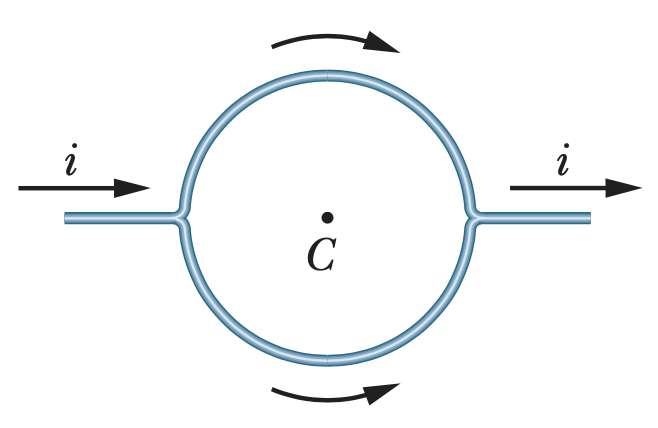
\includegraphics[scale=0.55]{qfig10-1.png}
  \caption{\textbf{문제 3}}
  \label{fig:3}
\end{figure}

\vspace{1cm}
\noindent {\bf 풀이 :} 
\vspace{1cm}

\noindent {\bf 문제 4 [50pt].}
그림~\ref{fig:4}은 반지름이 $a=4.00$ cm인 긴 원통형 도체에 반지름이
$b=1.50$ cm의 긴 원통형 구멍이 도체의 축과 평행되게 나 있는 걸
보여주는 단면이다.  이 구멍의 중심은 원형 도체의 중심에서부터 $d=2.00$
cm 떨어져 있다. 이 원통형 도체에는 전류 $i=5.25$ A가 균일하게 흐르고
있다고 하자. 
\begin{figure}[htp]
  \centering
  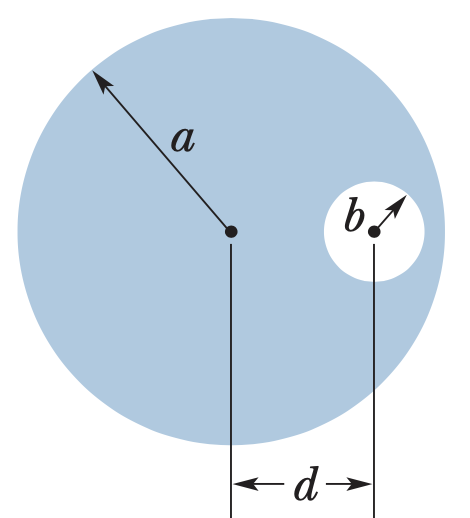
\includegraphics[scale=0.55]{qfig10-3.png}
  \caption{\textbf{문제 4}}
  \label{fig:4}
\end{figure}
\begin{itemize}
\item[(가)] 이 구멍의 중심에서 자기장은 얼마인가?
\item[(나)] $b=0$일 때와 $d=0$일 때의 결과를 구하고 논하여라. 
\end{itemize}

\vspace{1cm}
\noindent {\bf 풀이 :} 
\vspace{1cm}


\end{document}